\chapter{Potential Applications}
\label{ch:Applications}

After doing a study about the different systems to monitor and analyse the postural adjustments, we proceed to explain possible applications in the real life.

The force plate system is a very accurate system to analyse disorders in the patients, however it is a limited system for its price and portability. So, its applications make restricted to diagnosis some diseases.
The same happens with Qualisys System because it is necessary fixed cameras to record data. However it is a interesting way to observe data in real time with precision and robustness .

But, without a doubt, Gait Watch System is one of the most interesting system due to portability and its amount of fields where it can be used such as telerehabilitation, daily activities and performance of some athletics. This is why, the majority of applications will be focused in this system.

All of these implementations will be briefly explained below as well as a business idea as a concrete application of this Project.

\section{Diseases}
There exists a large amount of diseases that distort the motor control of human body or present symptoms that can be identified by the analysis of human body posture and motion. Along this section,  we will briefly comment how our study has influence in that.

\subsection{Neurological and Muscular diseases}
\textbf{Parkinson’s disease} is the second neurodegenerative disorder more frequent after Alzheimer\cite{AppPD}. According to the Parkinson’s disease fundation, PD is a chronic and progressive movement disorder, meaning that symptoms continue and worsen over time\cite{pdf}.
Many as one million Americans and 60,000 Spaniards and 10 million people worldwide live with Parkinson’s disease. Also, there is a large number of cases that go undetected \cite{A.Olivares2013}.

Primary motor signs of Parkinson’s disease include trembor, bradykinesia, dyskinesia and disorders in the posture and gait. Bradykinesia is the term for defining slow execution of the movement, tremor is the term used to define repetitive periodic movements within a certain frequency range and dyskinesia is a movement disorder which consists of effects including diminished voluntary movements and the presence of involuntary movements .Inertial Systems could be used to detect these disorder and help to diagnose and monitor them \cite{A.Olivares2013}.

Another disease associated to the central nervous system is \textbf{Multiple Sclerosis (MS)}. MS is an autoinmune disease characterize bay scar tissue resulting from the repair of damage to the myelin sheath that surronunds neurons. MS affects approximately 2.5 million people worlswide. Symptoms of MS are unpredictable but may inlcude fatigue, visión problems, loss of balance and coordination, or depression. Also, Individuals with MS often have por balance control that is especially apparent during dynamic task suach as gait initation. Hence, Inertial Sensors may be a useful tool to detect these symptoms \cite{Jebb2008}.


\textbf{Cerebral  palsy (CP)}is important to be mention  because it is a movement disorder appears in early childhood. CP is a neurodevelopmental condition caused by non-progressive brain lesión, can occur before, during or shortly after birth. Children diagnosed with CP demonstred increased muscle activity to sustain posture, agonist/antagonist co-contraction, impair postural control, inadecuate force production, and restrictive voluntary ans selective control of movement\cite{Gay2011}.

These impairments nor only interfere with performance of functional activities, but also with opportunities  ans/or willingness to participate in leisure, community ans achool activities.

Impaired postural control in CP includes difficulty organizing compensatory postural adjustments (CPAs) and anticipatory postural adjustments (APAs) \cite{Gay2011}. For that purpose,  consideration should be given to the use of Inertial Sensors to monitor this disease in dialy life.

\subsection{Sleep disorder}
\textbf{Sleep disorders} cause an unrestful sleep and important repercussions in some cases such as sleepiness and psychiatric and cardiorespiratory secondary disorders\cite{SanchezDaniel}. 

In order to diagnose them, we can use inertial sensors to monitor changes that occur during sleep. In addition, it is a good option to do this  cheap and portable, in such a way that patient can move freely while they are being monitored\cite{A.Olivares2013}.

Also, the information gathered can provide information  of the cardiac, respiratory, and snoring activities of patients sleeping\cite{SanchezDaniel}.

If we use all of this at home, it is possible to provide a tool to sleep specilists for knowing the behaviour of the patient when they are sleeping, what sleep cycles are more affected and improve their medical  treatments. 

For example,  some of the patients with \textbf{Epilepsy} suffer as tonic-clonic nocturnal seizures. These seizures  may go unnoticed to the patient, thus, during the control sessions with the doctor the patient could not tell the doctor these episodes. To avoid such a situation, the patient may sleep with an attached MIMU so nocturnal seizures can be detected and stored in the memory, allowing the doctor to notice that nocturnal attacks are happening\cite{A.Olivares2013}. 

\section{Dialy activities }
Providing new wereable technology for medical and surgical \textbf{rehabilitation} services is emerging as important option for clinicians and patients. Wereable technology like inertial sensors provides  a convenient platform to be able to quantify the long-term context and physiological response for  individuals\cite{Sung}.

In the first phase of the reabilitation program the patient have to move to the medical center for treatment. However, the second phase patient have to do low intensity exercices to stregthen  the muscles. This last task doesn’t require continuous  supervisión, thus, MARG systems can avoid the overcrowding of rehabilitation centers and patient can do the exercise at home comfortably\cite{A.Olivares2013}.

In addition, doctors can then supervise the sessions carried out by the patients by remotely checking the logs. Also, they could detect differents activity states, for example, knowing whether a person  is sleeping, driving or doing exercise\cite{A.Olivares2013}.

\textbf{Fall detection} is a important aspect during daily life of elderly people . It is very clear that falls are a serious health issue and that systems automatically detecting a fall and calling for help could be of great help to solve it. 

Moreover, there are applications for the motion analysis in \textbf{sport activities} by attaching sensors like accelerometers and gyroscopes onto the athletes ‘  body segments. For example, for a swimmer, the discrimination of the swimming styles and the segmentation of the underwater stroke phases could be achieved. In addition, the physiological response was also detected on the wrist acceleation when the swimmer was fatigued in analsis method the intensive training situation\cite{Yuji}.



\section{Business plan }
\subsection{Executive Summary}
SmartManagement claims to improve  the quality of life of elderly  people and with motion disorders. This system can detect falls and call emergency ambulance service as well as gathering data from the inertial sensors to analyse the postural adjustment and the differents movements and activities during the day. This information will be sent to a server, so the doctor can access this information  doing a medical monitoring of the patient and changing the treatment whether it is necessary.

To do this, we will use inertial sensors attached over legs, trunk and arms. This devices are more wearables and cheaper than other systems for gait analysis. This lets us making a cheap and comfortable design for our customers. The signal processing will be carried out by application in android that will communicate with the devices. At the same time, this application will transmit this information to the server.

The Gait analysis with inertial sensor is a innovate field specially in Spain where there are not companies in the market developing this kind of products. Population get older and their necessities grow being their monitoring and self-reliance increasingly important.
There are international companies such as ‘Gaitup’ whose main goal is to assessment of the gait  and fall detection. This is a important competence but firstly we will focus in domestic market and also we will provide improvements in price, communication and services.

To achieve that, we will contact with hospital and old people’s home as well as public institutions because we pretend that users only pay a portion of the cost of the product. Also, we want to find private investors providing them publicity in return for a investment.
We plan to establish presence in Internet and social networks to show our product. With this, people will be able to know what we do and how can improve their lives, those of their relatives and other loves one.

We can see a visual summary of this using a Model Canvas [Second appendix].

\subsection{Company Description}
\textbf{SmartManagement} is a technological-based company whose objetive is the implementation and development of completed system to monitor elderly people with motion disorders. The company is currently developing a research work and seeking to stablish its corporate identity in the medical product field.

Our method for developing businesses is ‘lean starup’, so the product is not closed, but we recieve information from our customers to improve the prototipe and provide their requirements.

The main motivations why this Project are impacts are:
-	As population age, health expenditures tend to grow rapidly since older persons usually require more health care in general and more specialized services to deal with their more complex pathologies(Stadistics from DESA,  World Population Ageing 2013\cite{desa}).

-	Globally, 40 per cent of older persons aged 60 years or over live independently. This indicate the necesity of continuous assistance(Stadistics from DESA,  World Population Ageing 2013\cite{desa}).

-	One of the most causes of disability and health problems in old age are falls and immobility (Stadistics from DESA,  World Population Ageing 2013\cite{desa}).

-	For the elderly who fall and are unable to get up on their own, the period of time spent immobile often affects their health outcome. Muscle cell breakdown starts to occur within 30-60 minutes of compression due to falling. Dehydration, pressure sores, hypothermia, and pneumonia are other complication that may result\cite{A.Olivares2013}.

The objetives of the company are as follows:
-	Improving the quality of life fo elderly people.
-	Making a Custom-made desing so it will be different and fit for each people.
-	Avoiding the overcrowding of old people’s home and hospitals.
-	Increasing the length of home stay where old people used to be more confortable.
-	Helping elderly people as well as people with motion disorders, increasing their self-reliance.
-	Establish a medical advisory board.

\subsection{Market Analysis}
 Over the past few decades the increased level of public awareness concerning healthcare, physical activities, safety and environmental sensing has created an emerging need for smart sensor technologies and monitoring devices able to sense, classify, and provide feedbacks to users’ health status and physical activities, as well as to evaluate environmental and safety conditions[article]. This makes the project more interesting and specially timely.
 
 The potential customers of SmartManagement are both domestic and foreign although we will focus in the last one.
 
 Domestic customers include hospitals, elderly people and people with motion disorders like Parkinson Disease or Cerebral Palsy. Also, we have to considers the key partners like public institutions, suppliers or University where there is a great research in this field.
  The foreign market includes many of the above segments but also includes key distributors such as inertial sensors distributor.
 
 This kind of products aren’t marketed in Spain. However, there are some institutions and companies working in similar investigations. Telefonica  together with UPC (Polytechnic University of Cataluña) had developed a inertial sensors-based system for monitoring Parkinson's motor symptoms\cite{rempark}.
 
 In the international market, there are several companies developing products for gait analysis and activity monitoring. The main competition is a Swiss company called ‘Gaitup’\cite{gaitup}. This comany was founded in 2013 in with the will to make products and solution for evaluating health and performance, based on wearable sensor technology.
 
 Gaitup develops products like ‘Gait Analysis’ whose goals are evaluation of the treatment, fall risk and motor symptoms assessment and feedback to the patient. Also, ‘Activity monotoring package’ allows the identification from long-term data,healthy status and  evaluation in home environment.
 
 However, \textbf{SmartManagement} is not only focused in the product, but also it seek the confort and the necessities of the custumers. Thus, it is realised a custom-made desing and adapted to economic status of our customers. Also, another added value is the realization of courses to teach the operation and advantages of the product.
 
 Intel and Michael L.Fox Foundation is working in wearable technology for Parkinson disease. They announced the development of sensor technology and analytics platform for Parkinson’s treatments and monitoring\cite{IntelAndMjf}. Although it is focused in Parkinson disease, it could be expanded to other diseases or fields. Also, this indicate the importance of this types of project and its social impact.


\subsection{Organization and Management}
SmartManagement will have a CEO, who will be  in charge of managing. Also, the company will have the next structure:

-	\textbf{Hardware Department}: this department is in charge of the design of the devices, i.e the types of sensors, their  positions  and market study of inertial sensors and new trends.

-	\textbf{Software Department}: this department is divided in two more. One of them will realise the signal processing and data analysis. The sencod one will carry out the mobile application to gather and process the data in real time and send a urgent message whether this is necessary( for example, a fall).

-	\textbf{Communications and servers Department}: data will be processed and sent to a Server for the doctor is able to obtain the results for adjusting the treatment.

-	\textbf{Marketing Department}: All information about the project will be shown in  social networks. We consider the activity in social networks is very important and one way to show the importance of this project and its possibilities.
In addition, we will make a Web Site that will be used to contact us and show our products and services.

-	\textbf{Administration Department}: this department will be in charge of the administratives topics such as possible investors, legal issues and economics tasks.

\begin{figure}[H]
	\centering
	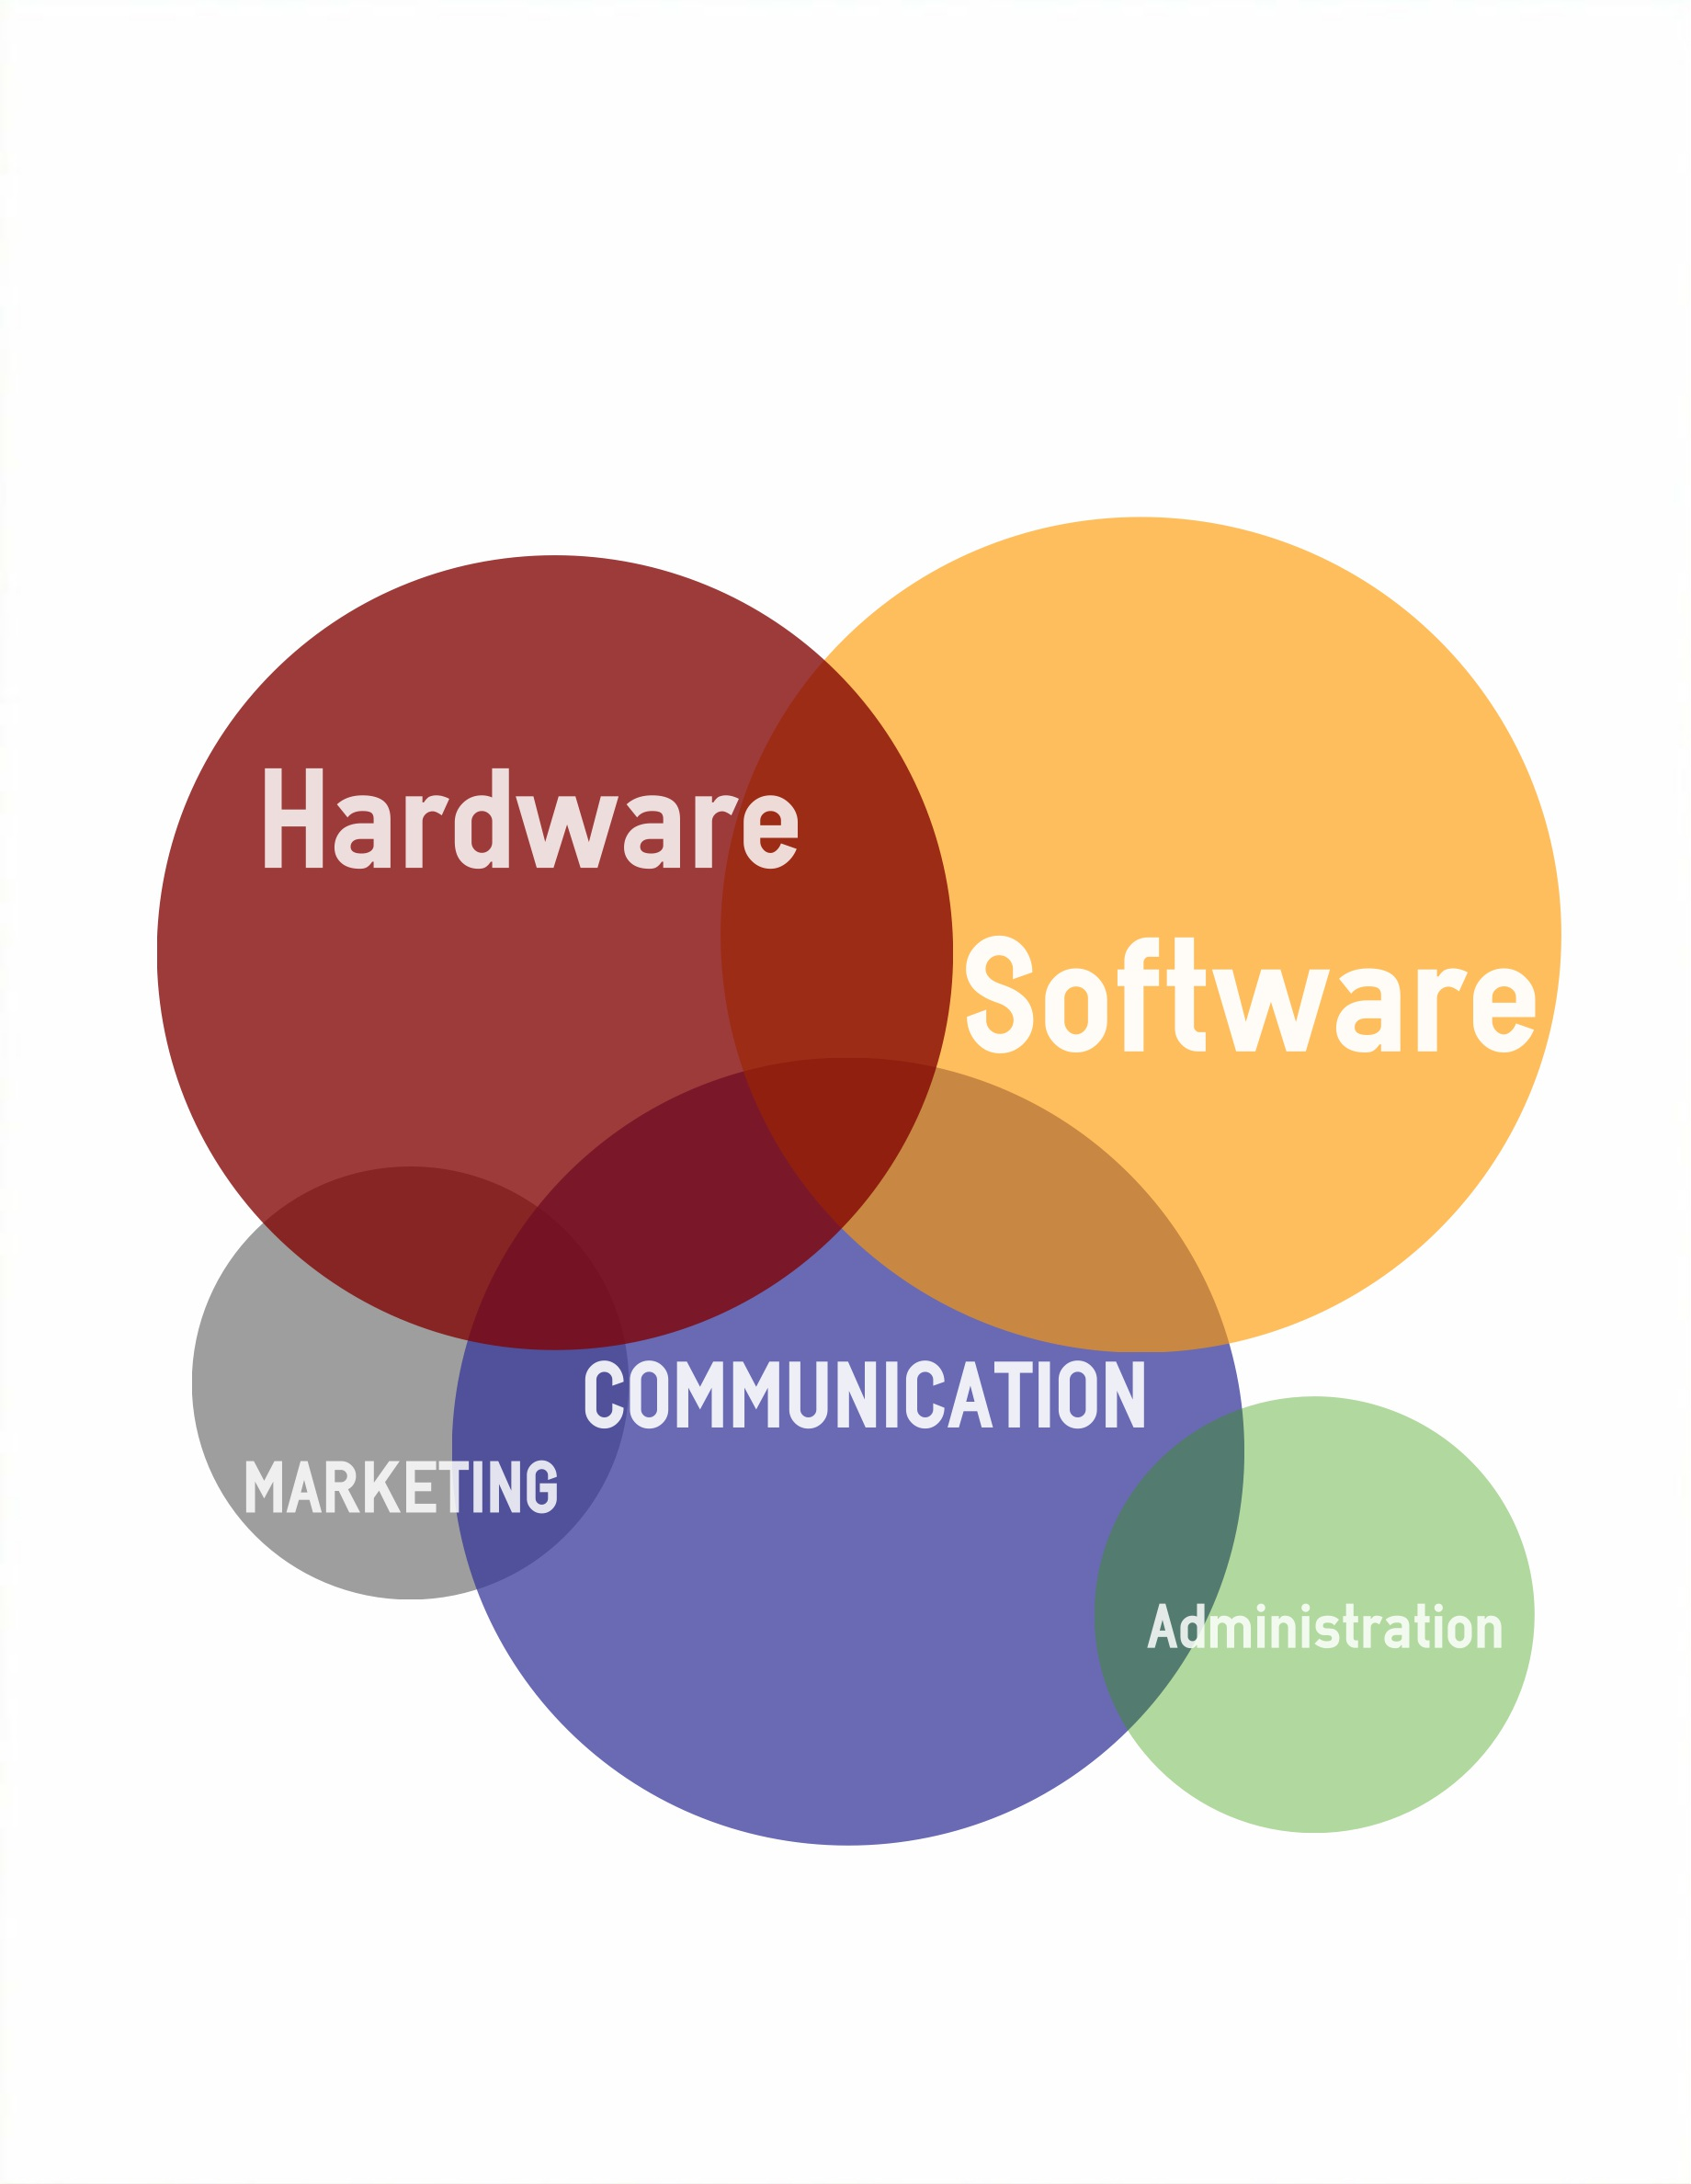
\epsfig{file=imagenes/Deparments, width=7cm}
	\caption{Diagram with the differents departments in the company.}
	\label{fig:Deparments}
\end{figure}

\subsection{Product Line}
The following is a brief explanation of the production process:

-	Assembling and configuration of inertial sensors. To do that, first we will obtain MEMs from ACAL bfi. Although there are a lot of supplier can provide these devices, we finally choose this one because it offers a great variability and quality in its products.

-	The next step is to use the signals from inertial sensors to carry out the signals processing and extract the main information to characterise the gait and others aspects such as falls or problems in the movement.

-	At the same time, we initially will do a application for mobile phone in Android and when this works properly, we would like to expand to iphone as well. The final idea is that everybody can use our product.

-	Then, we have to control the communication between inertial sensors and Smartphone as well as the communication between the mobile pone and cloud. We have to differentiate between the normal data transfer and urgent call. In the the first one, the data transfer between the Smartphone and cloud will send information to the server for afterwards the doctor can use this information and adjust the treatment of the patient. In the second one, the process is different because the mobile phone calls automatically to emergency department when person is at risk for fall or other similar situation.

-	Once we have a first prototype we are going to apply the ‘lean startup’ method. Some companies begin with an idea for a product that they think people want and after long time the company realise that customers don’t care about the idea. For this reason, we want to establish a feedback with our customers before of setting the final product, so  business will grow with maximum acceleration.

\begin{figure}[H]
	\centering
	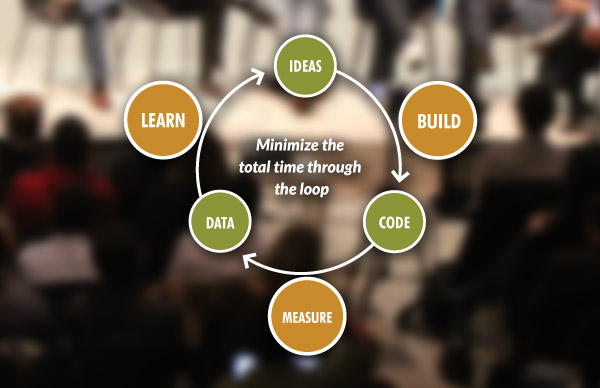
\epsfig{file=imagenes/leanstartup_diagram, width=7cm}
	\caption{Process of the 'lean startup' method.}
	\label{fig:leanstartup_diagram}
\end{figure}

\subsection{Marketing and Sales}
We will leverage a marketing and sales campaign because we are aware of firsts sales will be possible with a strong presence in social networks. The marketing strategy will have two phases. The first one is as follow:

-	Publicity in Internet. We will advertise on our Web Site and we also want to invest in google publicity for reaching people.

-	Building of Web Site. We will create a Web Site where we are going to show the description of our product and its possibilities to improve the quality of life for elderly people. Also, our customers will be able to buy the products here or contact us.

-	Publicity off-line. It will carry out using informatives meetings to show the advantages of this project. In addition, we will visit hospitals and old people`s home to inform personally.

-	Marketing on-line. Social network such as ‘twitter’ and ‘Facebook’ are a useful tools to advertise our products. Also, we pretend not only to show our advances but also keeping them actives publishing regularly.
We will use’ linkedin’ for providing employment and building a network outside contacts.
In addition, we will create a blog to give suggestion elderly people with motion disorders because we want to transmit our social engagement as well.

-	Presence in conferences, trade fairs and exhibitions.

Regarding sales strategy, these will sell on-line on the WebSite. However, we are aware  most of elderly people don’t use technologies, so we will use the hospitals and old people’s home to distribute the product. Also, we could send the product to their homes directly whether it is necessary.


\subsection{Finaltial projections}
Smart Management will be funded by a initial investment from the stockholders of the company and public institutions. It is important to develop awareness of the importance of this fact and obtaining grants to make the product.

We will need public grants because we consider that elderly people shouldn't pay a lot for this devices, so a part of the price will be funded by foundations and government and another by the user.

In addition, we are going to find investors for the project. They will be able to receive publicity and partners from our company. Thus, other goal for the company is to create a good relationship between partners and investors.

An amount of money achieved will be for hardware, software licenses, accommodation and marketing. The rest of the money will set aside for salaries of our employees. At the beginning the salary of the stockholders will depend on the company economy. After two or three years this will be adjusted, so they will have a fixed wage.


\subsection{SWOT Analysis}
\begin{figure}[H]
	\centering
	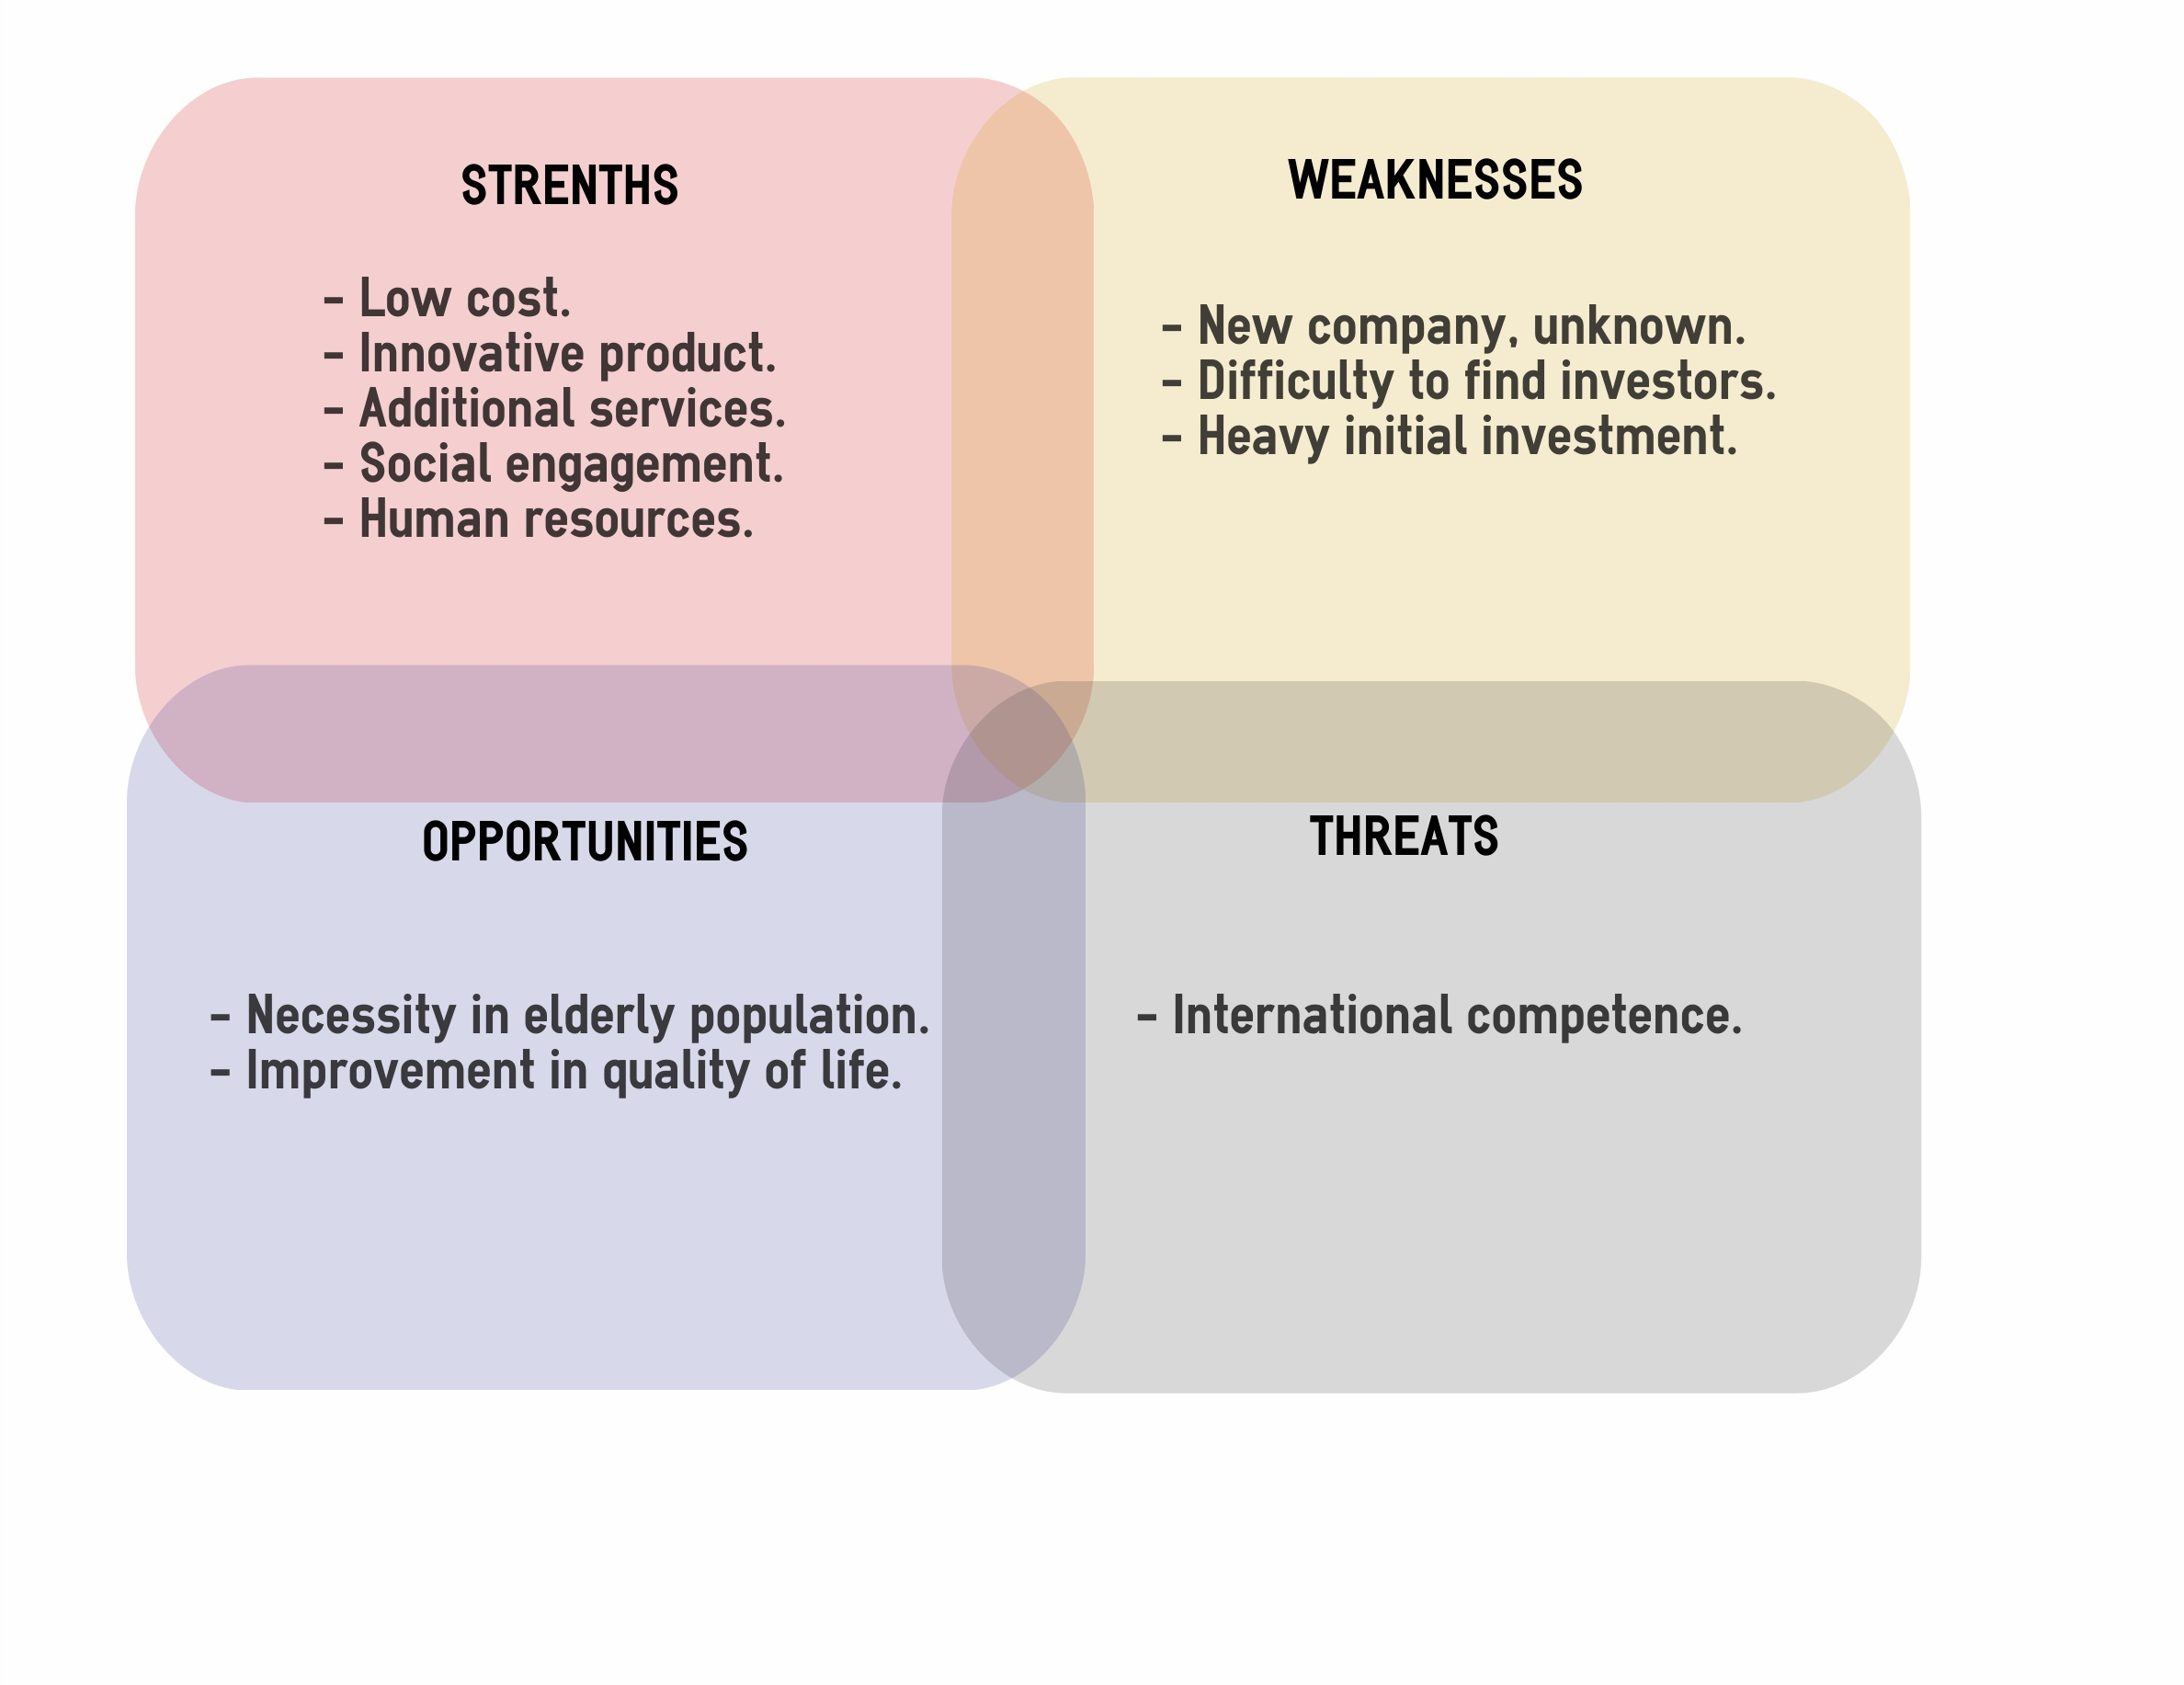
\epsfig{file=imagenes/SWOT, width=14cm}
	\caption{Table of the SWOT Analysis.}
	\label{fig:SWOT}
\end{figure}


